\appendix
\section{Appendix}
This section contains additional data and information that can be of interest to the readers but that are not strictly necessary for understanding the main text.

% \subsection{Publication Statistics Overview}
% \label{sub:publication_statistics}

% We conduct a thorough review of literature spanning from 2011 to 2023 to explore prevalent techniques (\textit{i.e.,} program analysis and patten discovery) in Android malware detection.
% Here, program analysis refers to the methods used to extract features from APK files, while pattern discovery involves the strategies employed to discern patterns from these features.

% To capture as many relevant studies as possible, we take search strategies used in~\cite{liu2022deep,liu2020review}. 
% Our literature search spanned major digital libraries, such as the ACM Digital Library and IEEE Xplore. 
% Throughout the search process, we mainly employ specific keywords to pinpoint relevant papers, including \texttt{android malware detection}, \texttt{android analysis}, and \texttt{android malware}.
% A further manual review of titles and abstracts allows us to filter out papers unrelated to our topic.
% Ultimately, this process yields 258 related papers.

% \begin{figure}[h]
%     \centering
%     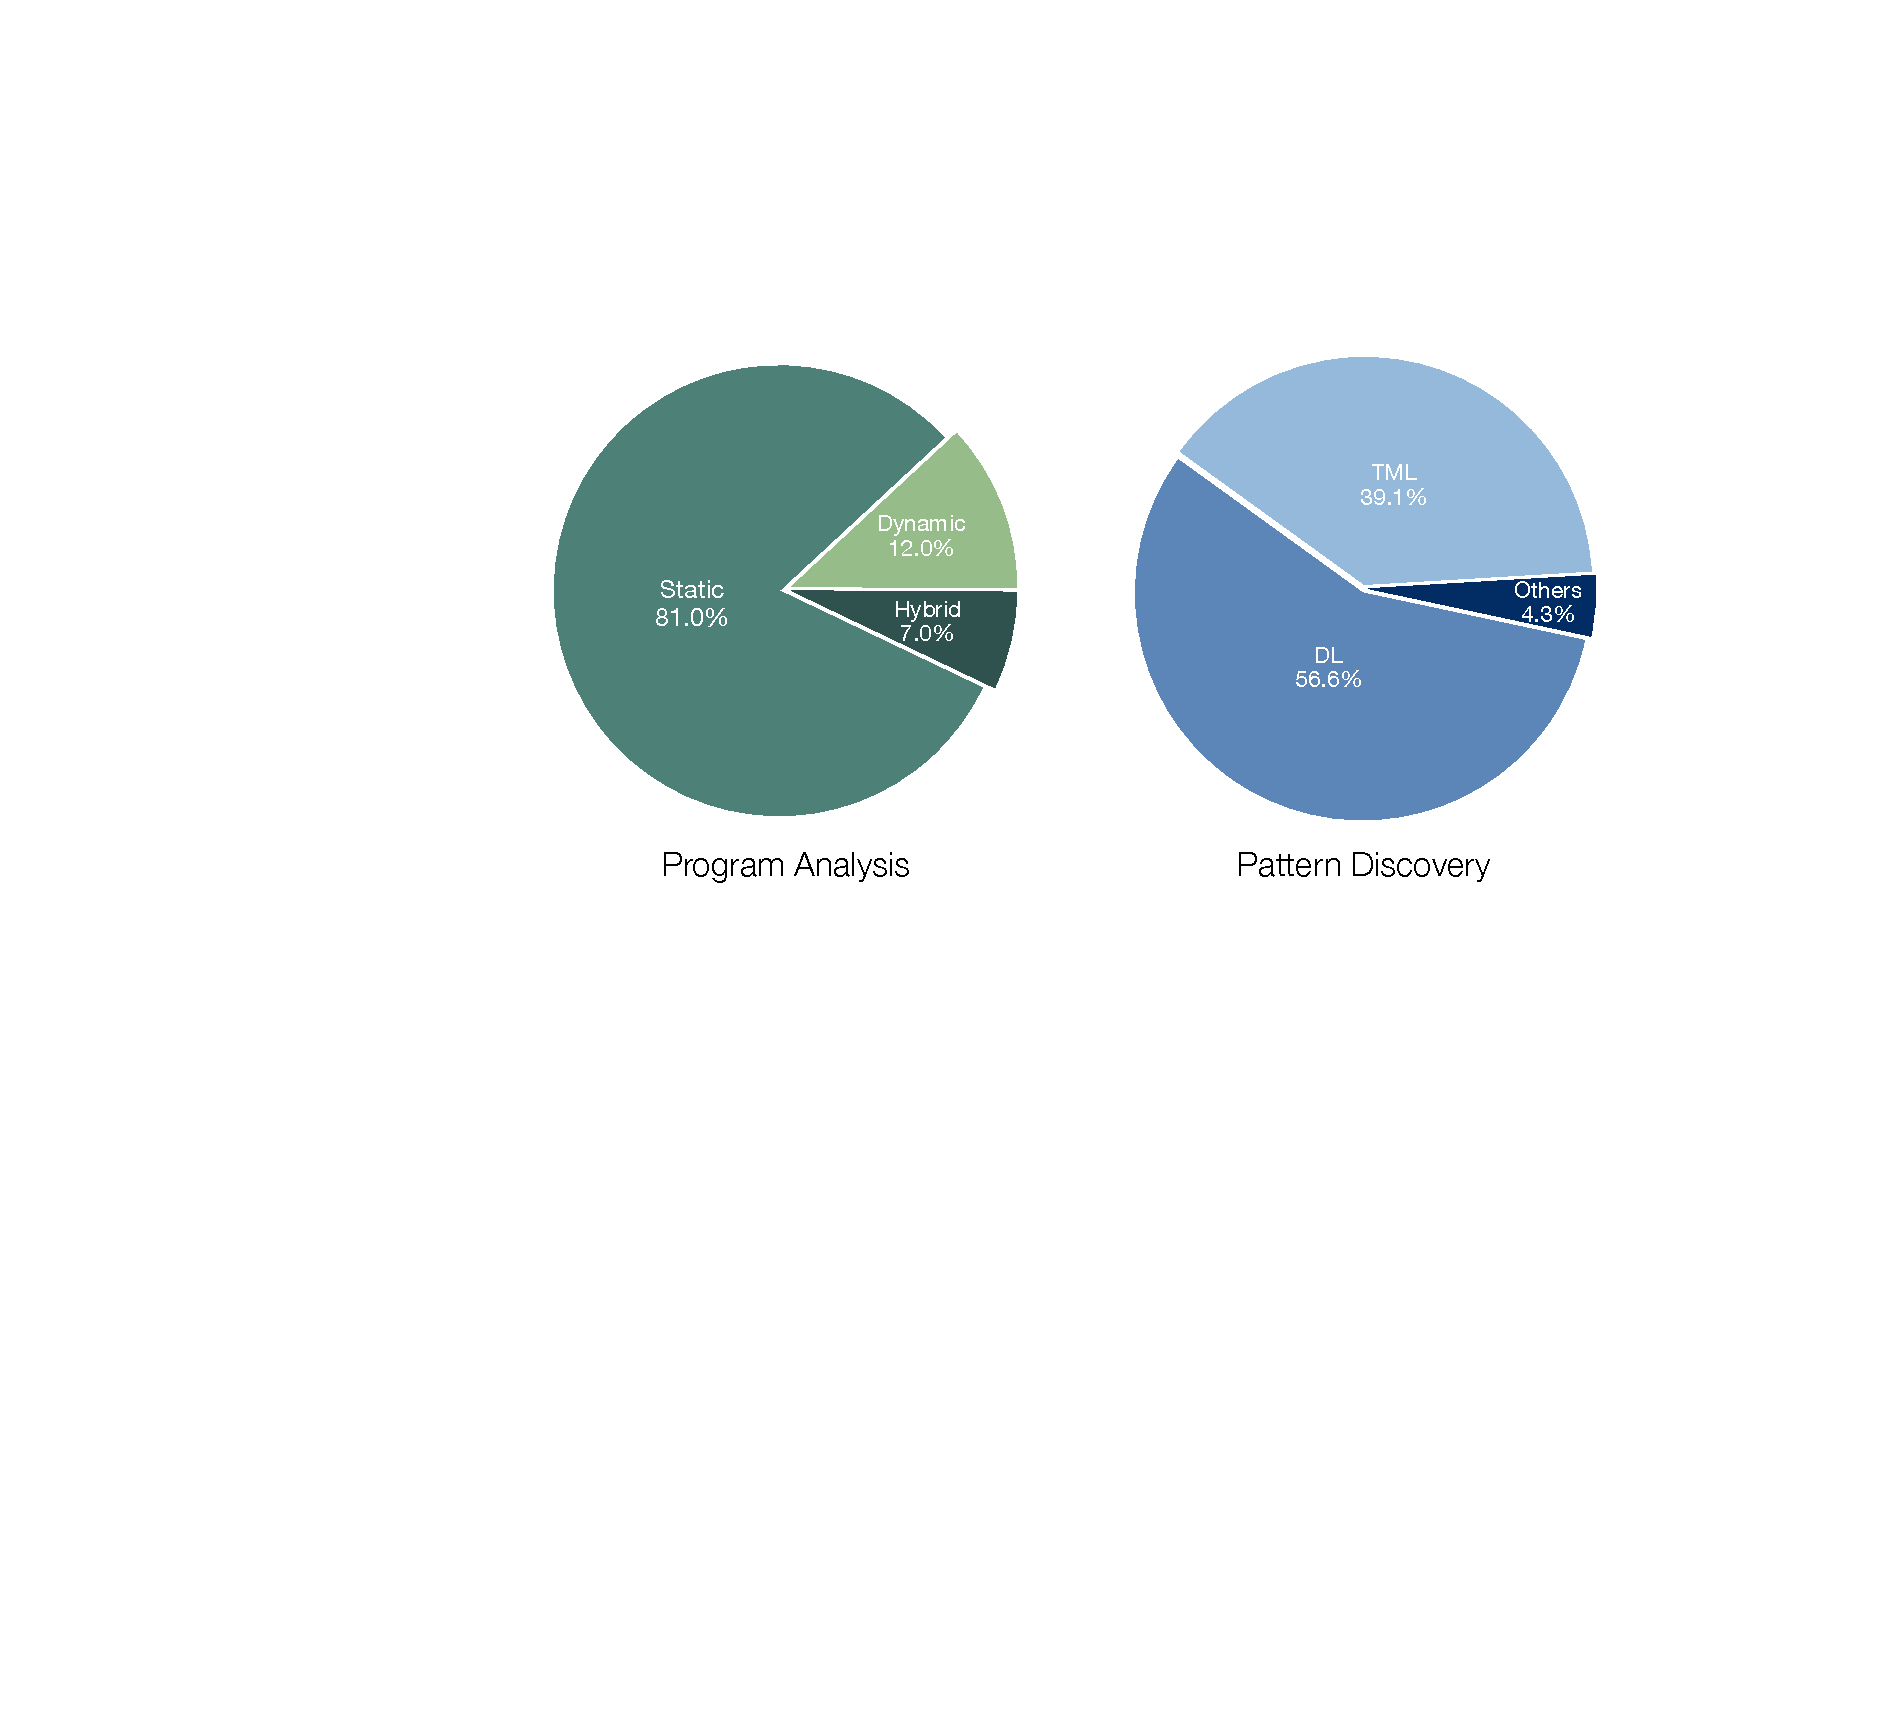
\includegraphics[width=0.73\linewidth]{fig/paper_distribution.pdf}
%     \caption{The overall distribution of investigated approaches from 2011 to 2023.}
%     \label{fig:paper_distribution}
%     \vspace{-0.3cm}
% \end{figure}


% We then categorize these papers based on the program analysis and pattern discovery techniques they employ.
% This distribution of these techniques is illustrated in Figure~\ref{fig:paper_distribution}.
% We observe that \textit{static analysis} emerges as the most favored program analysis technique, followed by \textit{dynamic analysis} and \textit{hybrid analysis}.
% Concurrently, \textit{machine learning (including both traditional machine learning and deep learning)} has been widely used to identify malware patterns.
% This observation further motivates us to focus on ML-based Android malware detection techniques that use static analysis.

\subsection{Feature Database}
\label{sub:feature_db}
To streamline the evaluation of different approaches, we establish a feature database to maintain commonly used features in Android malware detection.
Below, we outline the main features incorporated into the database, categorizing them for ease of reference.
\begin{itemize}[leftmargin=10pt]
    \setlength\itemsep{-1pt}
    \item \textit{Manifest}: this category contains features sourced from the \textit{AndroidManifest.xml} file, such as hardware components, permissions, intents, and app components.
    \item \textit{DisassembledCode}: this category includes the disassembled data extracted from the DEX file, such as the opcode, operands, and code strings.
    \item \textit{ProgramGraph}: this is mainly used to store the program graph of the APK file, including the nodes and edges.
    \item \textit{SharedLibrary}: this category contains the information of the shared libraries used by the APK file.
    \item \textit{Others}: this category includes other features that are not covered by the above categories.
\end{itemize}
Given the structure of the feature database, adding new features becomes straightforward, facilitating the adaptive evaluation of diverse approaches.
For instance, we can easily implement an add-on feature extractor and store the derived features in the database, waiting for use by the preprocessor.

% \vspace{-0.2cm}
% \subsection{\codename Implementation}
% \label{sub:implementation}
% \codename is developed in 17K lines of Python code.
% To ensure consistency and mitigate biases from different feature extraction toolchains and learning frameworks, we adopt standardized techniques across all tasks.
% For feature extraction, we use Androguard~\cite{androguard} to disassemble APK files and derive features such as permissions, intents, and program graphs. 
% LibRadar~\cite{libradar} helps in identifying third-party libraries within the applications, while Angr~\cite{angr} is used for analyzing native libraries and capturing essential features like opcodes and API calls. 
% When it comes to ML models, the scikit-learn library is our choice for traditional ML algorithms like SVM, KNN, and RF.
% On the other hand, for DL architectures such as CNN, GNN, and AE, we resort to Pytorch~\cite{pytorch}.
% This uniform approach ensures a balanced evaluation, concentrating purely on the uniqueness and performance of each method.

% \subsection{\codename Implementation}
% \label{sub:implementation}
% \codename is developed in 17K lines of Python code.
% To ensure consistency and mitigate biases from different feature extraction toolchains and learning frameworks, we adopt standardized techniques across all tasks.
% For feature extraction, we use Androguard~\cite{androguard} to disassemble APK files and derive features such as permissions, intents, and program graphs. 
% LibRadar~\cite{libradar} helps in identifying third-party libraries within the applications, while Angr~\cite{angr} is used for analyzing native libraries and capturing essential features like opcodes and API calls. 
% When it comes to ML models, the scikit-learn library is our choice for traditional ML algorithms like SVM, KNN, and RF.
% On the other hand, for DL architectures such as CNN, GNN, and AE, we resort to Pytorch~\cite{pytorch}.
% This uniform approach ensures a balanced evaluation, concentrating purely on the uniqueness and performance of each method.

\begin{table*}[t]
    \centering
    \caption{
    An overview of the 12 representative approaches we selected from major venues in security, software engineering, and machine learning. 
    \ymark \ indicates that the APK file (\textit{e.g.}, \textit{AndroidManifest.xml} for Manifest) is taken as input in Android malware detection, while \nmark \ is the opposite.
    \cmark \ and \xmark \ indicate whether feature engineering is handcrafted using domain knowledge or learned using representation learning.
    The effectiveness is based on the results reported in the original papers.}
    \vspace{-0.1cm}
    \begin{adjustbox}{width=\linewidth}
    \begin{tabular}{@{}c|cc|cccc|cc|rr|rrr@{}}
    \toprule
    \multirow{2}{*}{\raisebox{-0.3cm}{\textbf{\begin{tabular}[c]{@{}c@{}}Selected \\ Approach\end{tabular}}}} & \multicolumn{2}{c|}{\textbf{Publication}} & \multicolumn{4}{c|}{\textbf{Input from APK}} & \multicolumn{2}{c|}{\textbf{Feature Engineering}} & \multicolumn{2}{c|}{\textbf{Dataset}} & \multicolumn{3}{c}{\textbf{Effectiveness}} \\ \cmidrule(lr){2-3} \cmidrule(lr){4-7} \cmidrule(lr){8-9} \cmidrule(lr){10-11} \cmidrule(l){12-14}
     & \textbf{Venue} & \textbf{Year} & \textbf{Manifest} & \textbf{Dex} & \textbf{Resource} & \textbf{Library} & \textbf{Handcrafted} & \textbf{Learned} & \textbf{Malware} & \textbf{Goodware} & \textbf{TPR} & \textbf{FPR} & \textbf{F1} \\ \midrule
    Drebin\cite{arp2014drebin} & NDSS & 2014 & \ymark & \ymark & \nmark & \nmark & \cmark & \xmark & 5,560 & 123,453 & 94\% & \textbf{1\%} & 87\% \\ \midrule
    % ICCDetector\cite{xu2016iccdetector} & TIFS & 2016 & \ymark & \ymark & \nmark & \nmark & & & 5,264 & 12,026 & 93\% & \textbf{1\%} & 96\% \\ \midrule
    MamaDroid\cite{mariconti2016mamadroid} & NDSS & 2017 & \nmark & \ymark & \nmark & \nmark & \cmark & \xmark & 35,493 & 8,447 & 97\% & 2\% & 96\% \\ \midrule
    Mclaughlin et al.\cite{mclaughlin2017deep} & CODASPY & 2017 & \nmark & \ymark & \nmark & \nmark & \xmark& \cmark & 13,637 & 13,758 & 95\% & \textbf{1\%} & 97\% \\ \midrule
    HinDroid\cite{hou2017hindroid} & KDD & 2017 & \nmark & \ymark & \nmark & \nmark & \cmark & \xmark & 1,216 & 1,118 & \textbf{99\%} & 2\% & \textbf{99\%} \\ \midrule
    DeepRefiner\cite{xu2018deeprefiner} & EuroS\&P & 2018 & \ymark & \ymark & \ymark & \nmark & \xmark & \cmark & 62,915 & 47,525 & 98\% & 2\% & 98\% \\ \midrule
    Kim et al.\cite{kim2018multimodal} & TIFS & 2018 & \ymark & \ymark & \nmark & \ymark & \cmark & \cmark & 21,260 & 20,000 & \textbf{99\%} & \textbf{1\%} & \textbf{99\%} \\ \midrule
    MalScan\cite{wu2019malscan} & ASE & 2019 & \nmark & \ymark & \nmark & \nmark & \cmark & \xmark & 15,430 & 15,285 & --- & --- & 98\% \\ \midrule
    SDAC\cite{xu2020sdac} & TDSC & 2020 & \nmark & \ymark & \nmark & \nmark & \cmark & \cmark & 34,497 & 35,645 & 98\% & \textbf{1\%} & \textbf{99\%}\\ \midrule
    HomDroid\cite{wu2021homdroid} & ISSTA & 2021 & \nmark & \ymark & \nmark & \nmark & \cmark & \xmark & 3,358 & 4,840 & 97\% & 4\% & 95\% \\ \midrule
    Xmal\cite{wu2021android} & TOSEM & 2021 & \ymark & \ymark & \nmark & \nmark & \cmark & \xmark & 15,570 & 20,120 & 98\% & 2\% & 98\% \\ \midrule
    RAMDA\cite{li2021robust} & WWW & 2021 & \ymark & \ymark & \nmark & \nmark & \cmark & \xmark & 21,621 & 36,862 & 93\% & \textbf{1\%} & 90\% \\ \midrule
    MSDroid\cite{he2022msdroid} & TDSC & 2022 & \nmark & \ymark & \nmark & \nmark & \cmark & \xmark & 30,210 & 51,580 & 97\% & \textbf{1\%} & 97\% \\ \bottomrule
    \end{tabular}
    \end{adjustbox}
    \centering
    \begin{tablenotes}
    \footnotesize
    \item \ \ TPR, FPR, and F1 refer to true positive rate, false positive rate, and F1-score. 
    As MalScan is only evaluated on F1, its TPR and FPR are not available.
    \end{tablenotes}
    \label{tab:literature}
    \vspace{-0.3cm}
\end{table*}

\subsection{Reproduction of Selected Approaches}
\label{sub:approach_overview}
Table~\ref{tab:literature} offers a summary of the 12 representative approaches we have selected from leading publications in security~\cite{arp2014drebin,mariconti2016mamadroid,mclaughlin2017deep,xu2018deeprefiner,kim2018multimodal,xu2020sdac,he2022msdroid}, software engineering~\cite{wu2019malscan,wu2021homdroid,wu2021android}, and machine learning~\cite{hou2017hindroid,li2021robust}.
Within this table, we outline the publication details, input from APK, feature engineering style, dataset statistics, and their original effectiveness.
% As highlighted in Section~\ref{sec:discussion}, inconsistencies might exist between our quantitative evaluation results and those previously reported due to various biases, such as datasets, feature extraction toolchains, and learning frameworks.
To better support subsequent research and foster replicability and comparison, we provide the hyper-parameters of these approaches.

\bulletpoint{Drebin}
We replicate Drebin~\cite{arp2014drebin} utilizing a linear SVM with $C=1$, and set max number of iterations to $1000$.

\bulletpoint{MamaDroid}
MamaDroid~\cite{mariconti2016mamadroid} has two abstract mode \textit{i.e.}, package and family.
In our experiments, we choose the family mode, as it is more efficient in terms of time and memory.
For the RF classifier, we employ the default hyper-parameters provided by scikit-learn.

\bulletpoint{Mclaughlin et al}
Mclaughlin et al.~\cite{mclaughlin2017deep} is implemented with a CNN with one single convolutional layer, followed by a max-pooling layer and a fully connected layer.
The convolutional layer is configured with $32$ filters and a kernel size of $225*7$.
The fully connected layer has $16$ neurons.
For the evaluation process, a learning rate of $0.01$ and a batch size of $32$ are employed.
Additionally, inputs that exceed a length of $600000$ are truncated to $60000$, and those that are less than $600000$ are padded with zeros.

\bulletpoint{HinDroid}
In implementing HinDroid~\cite{hou2017hindroid}, various meta-path combinations have been tested. 
$AA^{T}$ yields remarkable performance in our experiments, and hence, is chosen as the meta-path.
For multi-kernel learning, we utilize the $p-norm$ multi-kernel learning framework as released by~\cite{sun2010multiple}, applying the default settings for the hyper-parameters.

\bulletpoint{DeepRefiner}
As discussed in Section~\ref{sub:selected_approaches}, DeepRefiner~\cite{xu2018deeprefiner} has two detection layers, and the second layer shows strong detection capability.
In our experiments, we replicate the second LSTM-based detection layer.
The model configuration is as follows: an embedding size of $16$ for word embeddings (bytecode instructions), a two-layer LSTM model with an input size of $16$, and a hidden size of $64$.
Batch size is set as $32$, and the learning rate is $0.001$.
The input sequence has a maximum length of $50,000$.
Inputs exceeding this length are truncated, while shorter inputs are padded with zeros.

\bulletpoint{Kim et al}
Kim et al.~\cite{kim2018multimodal} initially use a $5$ separated MLPs to process features from five various modalities, each with the same configuration.
Subsequently, a new MLP is introduced to integrate the learned features from the previous MLPs.
The initial five MLPs have layer configurations of $5000, 2500$, and $1000$ neurons.
The last MLP is structured with layers containing $1000, 500, 100$, and $10$ neurons, respectively.
A learning rate of $0.001$ and a batch size of $32$ are used during the training process.

\bulletpoint{MalScan}
The algorithm~\cite{wu2019malscan} is replicated with a KNN classifier, with the number of neighbors set to $3$.

\bulletpoint{SDAC}
SDAC~\cite{xu2020sdac} initially employs Word2Vec to encode API calls into vectors. Following this, K-means clustering is applied, and then these cluster centers are used as anchors to encode features.
In the classification phase, for simplicity, we use a linear SVM instead of multi-voting SVMs.
Additionally, due to K-means's randomness, the algorithm is executed $5$ times, and the average results are computed.
The size of Word2Vec embedding is set as $10$.
The chosen number of clusters is $1000$, and the SVM is configured using default parameters, allowing for $5000$ iterations.

\bulletpoint{HomDroid}
The approach~\cite{wu2021homdroid} is executed using a KNN classifier, with the number of neighbors set to $1$.

\bulletpoint{Xmal}
Xmal~\cite{wu2021android} is implemented using a 3-layer MLP with a hidden size of $64$.
An attention layer is also incorporated, utilizing an MLP with a hidden size of $158$.
The learning rate is set as $0.001$, and the batch size is $20$.

\bulletpoint{RAMDA}
RAMDA~\cite{li2021robust}'s architecture consists of two parts: autoencoder and classifier.
The encoder and decoder each consist of a 3-layer MLP with a hidden size of $600$.
The classifier is a 4-layer MLP with a hidden size of $600$.
During the training process, the autoencoder is trained first, and then the classifier is trained.
Configuration parameters are established with a learning rate of $0.001$, a batch size of $64$, and epochs set at $20$.
A pre-defined reconstruction loss of $30$ is used.
To constrain the loss, the positive weights are defined as $\lambda_1 = 10, \lambda_2 = 1, \lambda_3 = 10$.

\bulletpoint{MSDroid}
MSDroid~\cite{he2022msdroid} is implemented using a 3-layer GNN with a hidden size of $512$.
Subsequent to this, a 2-layer fully connected network with a hidden size of $512$ is used to classify the APKs.
The model's training parameters are set with a learning rate of $0.01$ and a batch size of $64$.

% \begin{figure}[t]
%     \centering
%     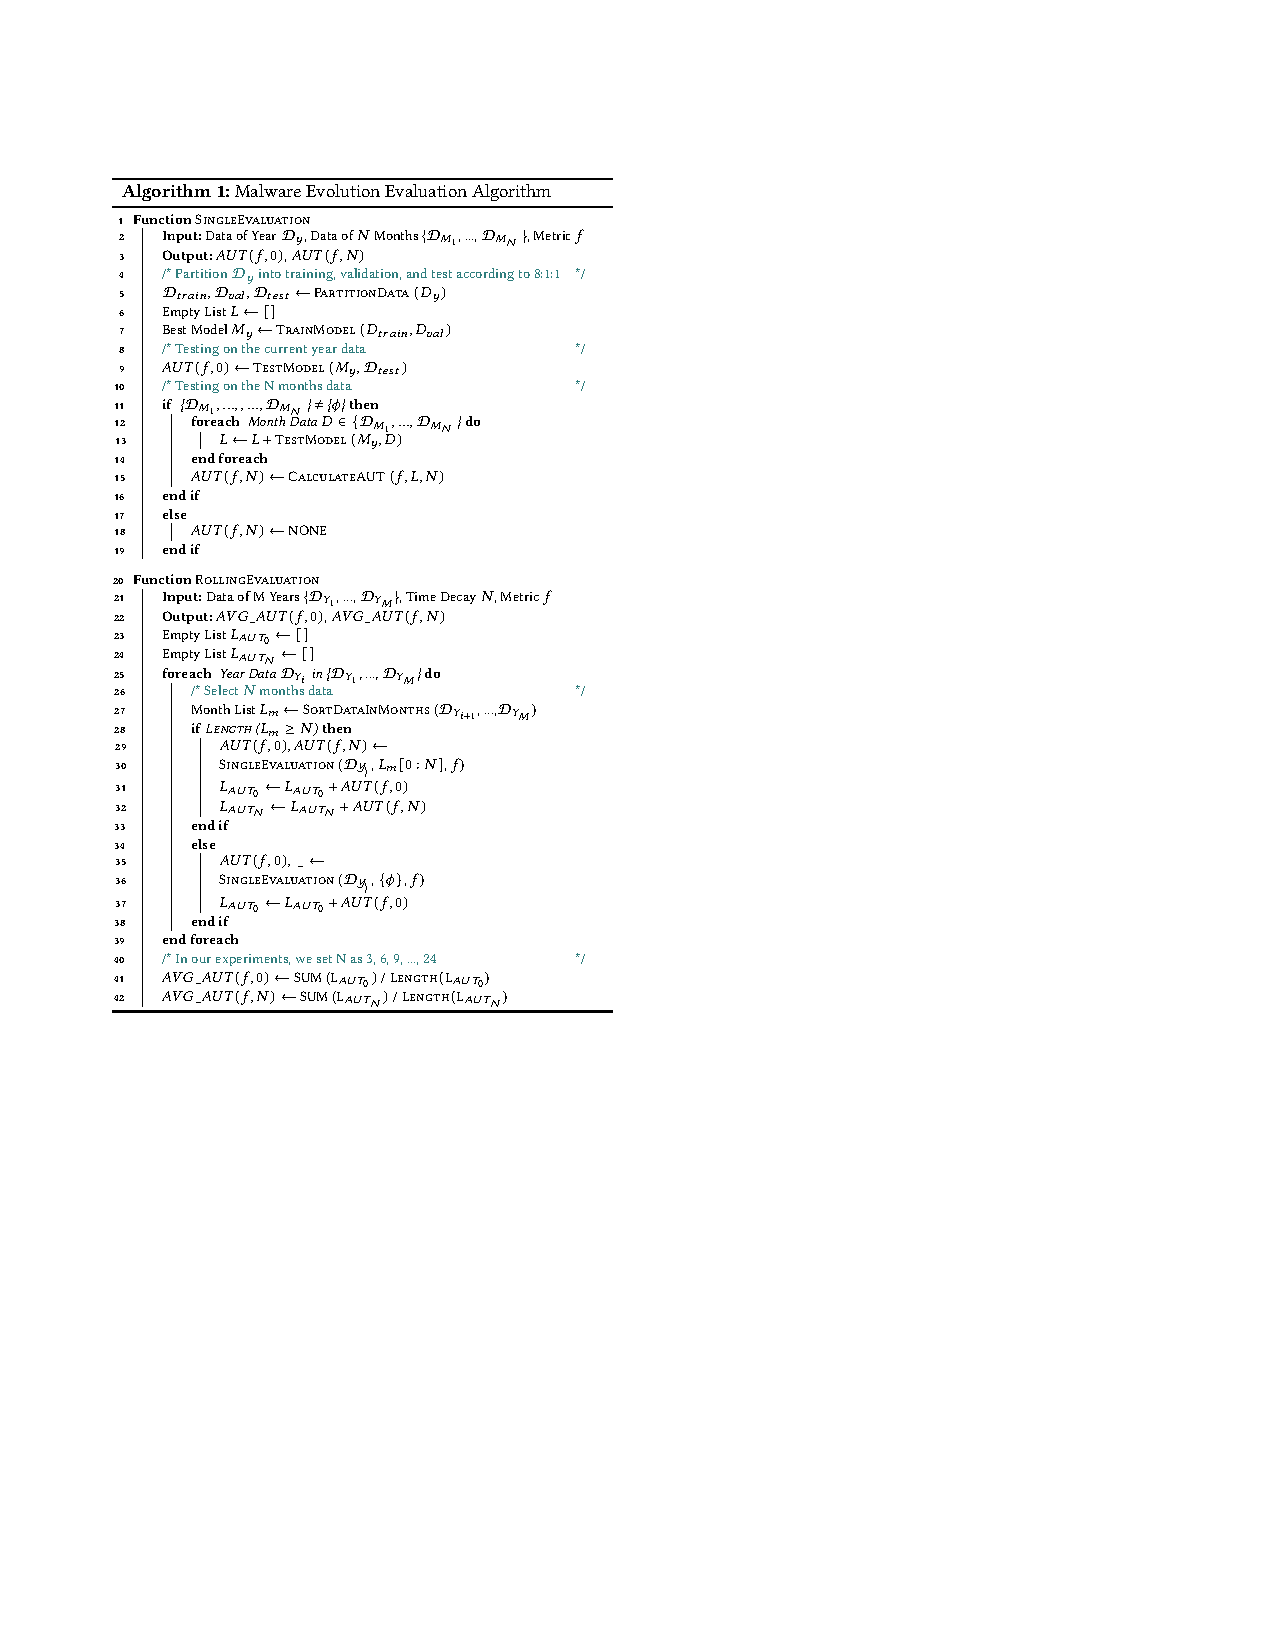
\includegraphics[width=0.86\linewidth]{fig/algorithm.pdf}
%     % \vspace{-0.3cm}
%     \caption{The rolling algorithm for evaluating the Android malware evolution.}
%     \label{fig:evolution_algorithm}
%     \vspace{-0.5cm}
% \end{figure}



\begin{table*}[t]
    \centering
    \renewcommand{\arraystretch}{1.1}
    \caption{The AUT(TPR, N) and AUT(FRP, N) of the selected approaches over varying time decays. In this analysis, we examine the shifts during various malware evolution periods: 3, 6, 9, 12, 15, 18, 21, and 24 months.}
    \vspace{-0.1cm}
    \begin{adjustbox}{width=\textwidth}
        \begin{tabular}{@{}c|c|c|c|c|c|c|c|c|c@{}}
            \toprule
            \textbf{Approach}         & \textbf{AUT(TPR,0)} & \textbf{AUT(TPR,3)} & \textbf{AUT(TPR,6)} & \textbf{AUT(TPR,9)} & \textbf{AUT(TPR,12)} & \textbf{AUT(TPR,15)} & \textbf{AUT(TPR,18)} & \textbf{AUT(TPR,21)} & \textbf{AUT(TPR,24)} \\ \midrule
            Drebin            & 0.803               & 0.722(-10.1\%)      & 0.670(-16.5\%)      & 0.601(-25.1\%)      & 0.564(-29.8\%)       & 0.530(-34.0\%)       & 0.508(-36.7\%)       & 0.484(-39.7\%)       & 0.466(-41.9\%)       \\ \midrule
            MamaDroid         & 0.712               & 0.496(-30.3\%)      & 0.429(-39.7\%)      & 0.365(-48.7\%)      & 0.322(-54.7\%)       & 0.308(-56.7\%)       & 0.282(-60.4\%)       & 0.253(-64.5\%)       & 0.233(-67.2\%)       \\ \midrule
            Mclaughlin et al. & 0.724               & 0.583(-19.6\%)      & 0.526(-27.3\%)      & 0.461(-36.4\%)      & 0.410(-43.4\%)       & 0.378(-47.9\%)       & 0.354(-51.2\%)       & 0.327(-54.9\%)       & 0.303(-58.1\%)       \\ \midrule
            HinDroid          & 0.831               & 0.786(-5.5\%)       & 0.773(-7.0\%)       & 0.729(-12.3\%)      & 0.687(-17.4\%)       & 0.684(-17.8\%)       & 0.674(-19.0\%)       & 0.662(-20.3\%)       & 0.655(-21.2\%)       \\ \midrule
            DeepRefiner       & 0.774               & 0.590(-23.7\%)      & 0.545(-29.6\%)      & 0.478(-38.3\%)      & 0.427(-44.8\%)       & 0.413(-46.6\%)       & 0.388(-49.9\%)       & 0.362(-53.2\%)       & 0.339(-56.2\%)       \\ \midrule
            Kim et al.        & 0.845               & 0.760(-10.0\%)      & 0.745(-11.8\%)      & 0.676(-20.0\%)      & 0.619(-26.7\%)       & 0.583(-31.0\%)       & 0.557(-34.0\%)       & 0.524(-38.0\%)       & 0.49(-42.0\%)        \\ \midrule
            MalScan           & 0.800               & 0.685(-14.4\%)      & 0.650(-18.8\%)      & 0.584(-27.0\%)      & 0.547(-31.6\%)       & 0.519(-35.2\%)       & 0.494(-38.3\%)       & 0.465(-41.8\%)       & 0.439(-45.1\%)       \\ \midrule
            SDAC              & 0.734               & 0.616(-16.1\%)      & 0.554(-24.5\%)      & 0.495(-32.6\%)      & 0.455(-38.0\%)       & 0.439(-40.2\%)       & 0.416(-43.4\%)       & 0.391(-46.8\%)       & 0.369(-49.7\%)       \\ \midrule
            HomDroid          & 0.836               & 0.689(-17.5\%)      & 0.651(-22.1\%)      & 0.596(-28.7\%)      & 0.546(-34.6\%)       & 0.515(-38.4\%)       & 0.486(-41.8\%)       & 0.448(-46.4\%)       & 0.422(-49.5\%)       \\ \midrule
            Xmal              & 0.836               & 0.741(-11.3\%)      & 0.693(-17.1\%)      & 0.617(-26.1\%)      & 0.575(-31.2\%)       & 0.550(-34.2\%)       & 0.523(-37.4\%)       & 0.492(-41.2\%)       & 0.463(-44.6\%)       \\ \midrule
            RAMDA             & 0.876               & 0.814(-7.0\%)       & 0.775(-11.6\%)      & 0.733(-16.3\%)      & 0.689(-21.3\%)       & 0.673(-23.2\%)       & 0.658(-24.8\%)       & 0.637(-27.2\%)       & 0.613(-30.1\%)       \\ \midrule
            MSDroid           & 0.835               & 0.755(-9.6\%)       & 0.732(-12.3\%)      & 0.673(-19.4\%)      & 0.635(-24.0\%)       & 0.632(-24.3\%)       & 0.604(-27.6\%)       & 0.569(-31.9\%)       & 0.544(-34.8\%)       \\ \midrule \midrule

            \textbf{Approach}         & \textbf{AUT(FPR,0)} & \textbf{AUT(FPR,3)} & \textbf{AUT(FPR,6)} & \textbf{AUT(FPR,9)} & \textbf{AUT(FPR,12)} & \textbf{AUT(FPR,15)} & \textbf{AUT(FPR,18)} & \textbf{AUT(FPR,21)} & \textbf{AUT(FPR,24)} \\ \midrule
            Drebin            & 0.014               & 0.02(+42.2\%)       & 0.023(+68.2\%)      & 0.024(+71.1\%)      & 0.026(+85.6\%)       & 0.029(+110.1\%)      & 0.030(+115.2\%)      & 0.031(+126.7\%)      & 0.033(+141.2\%)      \\ \midrule
            MamaDroid         & 0.009               & 0.010(+17.9\%)      & 0.011(+28.4\%)      & 0.010(+20.2\%)      & 0.011(+31.9\%)       & 0.013(+50.5\%)       & 0.013(+54.0\%)       & 0.014(+62.2\%)       & 0.014(+59.9\%)       \\ \midrule
            Mclaughlin et al. & 0.013               & 0.010(-19.1\%)      & 0.012(-7.5\%)       & 0.013(+1.9\%)       & 0.015(+14.3\%)       & 0.016(+23.6\%)       & 0.016(+24.4\%)       & 0.016(+22.1\%)       & 0.016(+20.5\%)       \\ \midrule
            HinDroid          & 0.016               & 0.262(+1491.6\%)    & 0.266(+1516.6\%)    & 0.271(+1548.8\%)    & 0.279(+1599.3\%)     & 0.319(+1839.1\%)     & 0.321(+1853.7\%)     & 0.324(+1873.8\%)     & 0.327(+1890.3\%)     \\ \midrule
            DeepRefiner       & 0.017               & 0.019(+9.3\%)       & 0.018(+5.9\%)       & 0.019(+7.6\%)       & 0.021(+20.3\%)       & 0.022(+27.2\%)       & 0.022(+28.9\%)       & 0.023(+31.2\%)       & 0.024(+38.7\%)       \\ \midrule
            Kim et al.        & 0.014               & 0.017(+19.7\%)      & 0.018(+29.8\%)      & 0.018(+31.9\%)      & 0.02(+43.5\%)        & 0.024(+75.9\%)       & 0.026(+84.6\%)       & 0.027(+91.8\%)       & 0.027(+95.4\%)       \\ \midrule
            MalScan           & 0.025               & 0.029(+17.1\%)      & 0.029(+18.7\%)      & 0.029(+17.9\%)      & 0.031(+24.8\%)       & 0.031(+26.1\%)       & 0.033(+33.0\%)       & 0.035(+40.7\%)       & 0.037(+50.1\%)       \\ \midrule
            SDAC              & 0.024               & 0.042(+72.1\%)      & 0.050(+104.4\%)     & 0.054(+121.6\%)     & 0.060(+146.5\%)      & 0.064(+159.6\%)      & 0.066(+169.9\%)      & 0.068(+176\%)        & 0.072(+192.3\%)      \\ \midrule
            HomDroid          & 0.014               & 0.023(+63.2\%)      & 0.024(+66.0\%)      & 0.023(+59.0\%)      & 0.024(+66.0\%)       & 0.026(+78.5\%)       & 0.028(+94.6\%)       & 0.031(+112.7\%)      & 0.032(+123.8\%)      \\ \midrule
            Xmal              & 0.023               & 0.025(+11.6\%)      & 0.028(+23.5\%)      & 0.027(+20.4\%)      & 0.027(+18.2\%)       & 0.028(+21.7\%)       & 0.028(+25.3\%)       & 0.029(+28.4\%)       & 0.030(+30.6\%)       \\ \midrule
            RAMDA             & 0.054               & 0.061(+14.0\%)      & 0.069(+27.6\%)      & 0.075(+38.7\%)      & 0.081(+50.0\%)       & 0.09(+67.1\%)        & 0.093(+73.4\%)       & 0.099(+84.2\%)       & 0.104(+93.9\%)       \\ \midrule
            MSDroid           & 0.072               & 0.078(+8.4\%)       & 0.080(+11.7\%)      & 0.082(+14.5\%)      & 0.085(+18.4\%)       & 0.093(+29.2\%)       & 0.098(+37.3\%)       & 0.106(+47.4\%)       & 0.111(+55.1\%)       \\ \bottomrule
            \end{tabular}
    \end{adjustbox}
    \label{tab:tpr_time_decay}
    \vspace{-0.3cm}  
\end{table*}

\begin{table}[t]
    \centering
    \renewcommand{\arraystretch}{0.6}
    \caption{The effectiveness of the selected approaches using different size training data.}
    \vspace{-0.1cm}
    \begin{adjustbox}{width=0.54\linewidth}
    \begin{tabular}{@{}c|c|c|c@{}}
    \toprule
    \diagbox[innerleftsep=-0.1em, innerrightsep=-0.2em, height=2.6em,width=7em]{\textbf{Approach}}{\textbf{Data Size}} & \textbf{100\%} & \textbf{50\%}& \textbf{10\%}\\ \midrule
    Drebin& 0.722 & 0.714 (-1.2\%) & 0.643 (-10.9\%) \\ \midrule
    MamaDroid& 0.661 & 0.623 (-5.7\%) & 0.452 (-31.5\%) \\ \midrule
    Mclaughlin et al.& 0.714 & 0.627 (-12.2\%) & 0.140 (-80.4\%) \\ \midrule
    HinDroid & 0.731 & 0.716 (-2.0\%) & 0.618 (-15.5\%) \\ \midrule
    DeepRefiner& 0.657 & 0.577 (-12.1\%) & 0.327 (-50.2\%) \\ \midrule
    Kim et al. & 0.782 & 0.742 (-5.1\%) & 0.611 (-21.8\%) \\ \midrule
    MalScan& 0.684 & 0.653 (-4.6\%) & 0.526 (-23.1\%) \\ \midrule
    SDAC & 0.522 & 0.496 (-5.0\%) & 0.474 (-9.1\%) \\ \midrule
    HomDroid& 0.734 & 0.675 (-8.0\%) & 0.586 (-20.1\%) \\ \midrule
    Xmal& 0.698 & 0.668 (-4.2\%) & 0.613 (-12.2\%) \\ \midrule
    RAMDA& 0.636 & 0.614 (-3.4\%) & 0.547 (-14.0\%) \\ \midrule
    MSDroid& 0.648 & 0.563 (-13.0\%) & 0.424 (-34.6\%) \\ \bottomrule
    \end{tabular}
    \end{adjustbox}
    \label{tab:res_training_size}
    \vspace{-0.3cm}
\end{table}

\subsection{AUT, ASR, and APR}
\label{sub:aut}
In assessing a classifier's resilience against temporal degradation, we employ the Area Under Time (AUT) metric as suggested by~\cite{pendlebury2019tesseract}.
AUT is formally given by:
$$
AUT(f, N) = \frac{1}{N-1}\sum_{k=1}^{N-1}\frac{f(k+1)+f(k)}{2},
$$
where $f$ represents the chosen performance metric (such as F1 score or True Positive Rate) and $N$ denotes the count of malware evolution period. 
AUT values range between $(0,1)$, where 1 indicates the classifier retains consistent performance across time.

To evaluate a classifier's robustness against adversarial attacks, we use two primary metrics: the attack success rate (ASR) and average perturbation ratio (APR) metrics utilized by~\cite{li2023black}.
They are mathematically defined as:
$$
ASR = \frac{N_{success}}{N_{total}}, \ APR = \frac{F_{modified}}{F_{total}}.
$$
Here, $N_{success}$ refers to the number of adversarial examples that successfully deceive the classifier.
$N_{total}$ represents the entire set of adversarial samples.
Meanwhile, $F_{modified}$ is the number of input features changed by the adversarial intervention, and $F_{total}$ signifies the total number of features in the input.
The ASR values fall within the interval $(0,1)$; a value of 1 suggests the classifier is entirely susceptible to adversarial attacks.
Similarly, APR values lie within $(0,1)$.
A higher APR indicates that evading the classifier becomes increasingly challenging.

% \vspace{-0.2cm}
% \subsection{Malware Evolution Algorithm}
% \label{sub:malware_evolution_algorithm}
% To evaluate the evolution of Android malware, we propose a rolling algorithm, as illustrated in Figure~\ref{fig:evolution_algorithm}.
% In our experiment, we use the data from 2011 to 2020, and the malware evolution periods are set as 3, 6, 9, 12, 15, 18, 21, and 24 months.

% \vspace{-0.2cm}
\subsection{Additional Results}
\label{sec:additional_results}
Table~\ref{tab:res_training_size} presents the detailed results of training data size analysis.
In Sec.~\ref{effectiveness}, we normalize the results of the selected approaches based on the use of 100\% training data size for clarity.
For instance, the normalized result for Drebin, using 50\% of the training data, is computed as $\frac{0.714}{0.722} = 0.988$.
These results highlight the significant impact that the volume of data has on the effectiveness of the selected approaches.

For the analysis of malware evolution, the results of AUT(TPR, N) and AUT(FPR, N) are reported in Table~\ref{tab:tpr_time_decay} (N is also set as 0, 3, 6, 9, 12, 15, 18, 21, and 24 months).
We observe that as malware evolution time increases, there is a consistent decrease in AUT(TPR, N) for the selected approaches.
This trend suggests that as malware evolves, more malware samples are misclassified as benign.
Simultaneously, an increase in AUT(FPR, N) is noted, indicating that more benign samples are misclassified as malware.
Overall, the performance of malware detection approaches degrades with the increase of malware evolution time.
